\documentclass[tikz,border=10pt]{standalone}
\begin{document}
% Pixel coordinates (y flipped), scaled so the longest side is about 8 cm
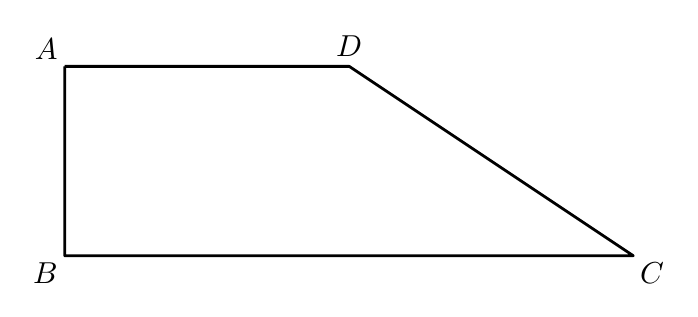
\begin{tikzpicture}[x=0.012719cm, y=0.012719cm, line width=1.0pt, line join=round]
  % Vertices (px, y flipped)
  \coordinate (A) at (68,-65);
  \coordinate (D) at (352,-65);
  \coordinate (C) at (635.5,-254);
  \coordinate (B) at (68,-254);

  % Solid outline: top, diagonal to C, bottom, left side
  \draw (A) -- (D) -- (C) -- (B) -- (A);

  % Labels (outside the figure)
  \node[above left, inner sep=2pt, font=\fontsize{10.5}{12.6}\selectfont] at (A) {$A$};
  \node[above, inner sep=3pt, font=\fontsize{10.5}{12.6}\selectfont] at (D) {$D$};
  \node[below left, inner sep=2pt, font=\fontsize{10.5}{12.6}\selectfont] at (B) {$B$};
  \node[below right, inner sep=2pt, font=\fontsize{10.5}{12.6}\selectfont] at (C) {$C$};
\end{tikzpicture}
\end{document}